\section{多视角下的中医治未病}
\begin{frame}{预防医学视角}
\begin{quote}
    健康:一个人生理上、心理上和社会上的完好状态。
    
    21世纪的医学,不应继续以疾病为主要研究对象,而应以人类健康作为医学研究的主要方向。
\end{quote}

\begin{block}{预防医学特点}
    \begin{itemize}
        \item 三级预防体系
        \item 依托西医学科背景,针对具体疾病
        \item 发展出流行病学、医学统计学等分支学科
    \end{itemize}
\end{block}
\end{frame}

\begin{frame}{预防医学视角}
\begin{quote}
    “夫病已成而后药之,乱已成而后治之,譬犹渴而穿井,斗而铸锥,不亦晚乎! ”《素问·四气调神论》
\end{quote}

\begin{block}{治未病特点}
    \begin{itemize}
        \item 三个层次(未病先防--既病防传--病后防复)
        \item 依托中医学科背景,针对个人和复杂情况
        \item 个人为实践主体,多层次多样化的实践手段
    \end{itemize}
\end{block}
\end{frame}

\begin{frame}{预防医学和治未病异同}
\begin{spacing}{1.19}

\begin{table}[]
    \begin{tabular}{|
            >{\columncolor[HTML]{FFFFFF}}c |
            >{\columncolor[HTML]{FFFFFF}}c |
            >{\columncolor[HTML]{FFFFFF}}c |}
        \hline
        & 预防医学      & 治未病         \\ \hline
        实践主体 & 卫生机构      & 机构/个人       \\ \hline
        实践方法 & 固定完整的操作流程 & 多层次多样化的实践方法 \\ \hline
        预防体系 & 三级预防      & 三级预防        \\ \hline
        预防内容 & 针对具体疾病    & 针对不同个体      \\ \hline
    \end{tabular}
\end{table}
\end{spacing}
\begin{exampleblock}{核心要点}
    预防医学强调流程化的操作,用概率/统计来评估效果;治未病则将主体转移到个人,强调这一理念植入生活。
\end{exampleblock}
\end{frame}

\begin{frame}[allowframebreaks]{国家政策视角}
\begin{block}{2013}
《中医预防保健(治未病)服务科技创新纲要(2013-2020年)》提出, 建设科普知识宣传队伍和网络,拓展信息渠道,鼓励以多种形式传播中医预防保健(治未病)服务文化和知识,加强中医预防保健(治未病)服务科技创新成果的知识普及,提高行业内外对中医预防保健(治未病)服务科技创新发展重要性的认识。
\end{block}
\begin{block}{2016}
   《“健康中国2030”规划纲要》提出,实施中医治未病健康工程,将中医药优势与健康管理结合,探索融健康文化、健康管理、健康保险为一体的中医健康保障模式……为群众提供中医健康咨询评估、干预调理、随访管理等治未病服务。
\end{block}
\begin{exampleblock}{2018}
2018年4月28日,国务院发布《国务院办公厅关于促进“互联网+医疗健康”发展的意见》,其中第六条第三项提出,建立网络科普平台,利用互联网提供健康科普知识精准教育,普及健康生活方式,提高居民自我健康管理能力和健康素养。
\end{exampleblock}
\end{frame}
\section{项目流程设计}
\begin{frame}{调研部分}
\begin{enumerate}
    \item 对20名社区居民进行访谈,目的在于了解居民健康需求、社区健康宣传和实际服务,居民获知信息渠道、居民关注的养生话题和日常养生行为。
    \item 设计相应知识、信念、行为三维度的问卷题目,并交予相关专家评议通过。
    \item 发放问卷,回收分析,撰写统计报告。
\end{enumerate}
\end{frame}
\begin{frame}{干预部分}
\begin{enumerate}
    \item 建立微信公众号,确定受众、选题范围和相关传播策略。
    \item 招募实验被试人员,通过初期情况统计/IP追踪等方法研究受干预群体的知信行情况。
    \item 进行随机化分组,对实验组进行为期三个月的推送,分析结果
\end{enumerate}
\begin{figure}[th]
    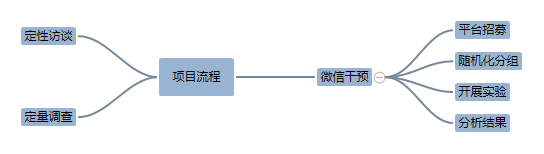
\includegraphics[width=\textwidth]{newprocess.png}
    \centering
    \caption{项目设计简图}
\end{figure}
\end{frame}
\section{调研部分报告}
\begin{frame}{定性结果分析}
通过定性访谈得出以下总体结论:
\begin{enumerate}
    \item 人群对于治未病意识较为薄弱,和经济水平和观念意识相关。
    \item 治未病作为具体的实践项目在不同的机构扮演不同的角色,在社区卫生服务中心大多以治疗项目出现,在居委会成为零散的宣传项目。
\end{enumerate}
\end{frame}
\begin{frame}{角色的分化}
\begin{alertblock}{结论分述}
\begin{enumerate}
\item 居民:遇病求医现象突出;基于经济考虑,保健意识较薄弱

\item 社区医院:接待人群多为老人儿童;资金定额;治未病项目散列

\item 居委会:网格制度联系居民;治未病范畴宣教;慢病管理。
\end{enumerate}
\end{alertblock}
\end{frame}
\begin{frame}{几个待探究的问题}
\begin{exampleblock}{待探究问题}

\begin{enumerate}
    \item 更普遍条件下居民对中医治未病的知识、信念、行为情况
    \item 上述情况和居民性别、年龄、教育、收入等的联系
\end{enumerate}\end{exampleblock}
\begin{alertblock}{问卷调研}
    我们在南京市五福家园社区、东方城社区、兴隆社区、华侨路社区、凤凰二村社区发放先行设计的知信行问卷,共回收265份。统计分析如下:
\end{alertblock}
\end{frame}

\begin{frame}[allowframebreaks]{定量结果分析}
\begin{columns}
\begin{column}{0.7\textwidth}
    \begin{block}{各题维度、类型、跳题设置}
\begin{longtable}[]{@{}llll@{}}
    
    题号 & 维度 & 题目类型 & 是否有跳题\tabularnewline
    \hline
    \endhead
    1 & 知识 & 单选 & 是\tabularnewline
    2 & 知识 & 多选 & 否\tabularnewline
    3-10 & 知识 & 单选 & 否\tabularnewline
    11 & 知识 & 多选 & 否\tabularnewline
    12-19 & 信念 & 单选 & 否\tabularnewline
    20 & 行为 & 单选 & 是\tabularnewline
    21 & 行为 & 多选 & 否\tabularnewline
    22-26 & 行为 & 单选 & 否\tabularnewline
    \hline
\end{longtable}
\end{block}
\end{column}
\begin{column}{0.6\textwidth}
\begin{block}{分类变量}
\begin{longtable}[]{@{}lll@{}}
    
    题号 & 变量名称 & 类型\tabularnewline
    \hline
    \endhead
    27 & 性别 & 分类\tabularnewline
    28 & 年龄 & 数值\tabularnewline
    29 & 学历 & 分类\tabularnewline
    30 & 年收入 & 分类\tabularnewline
    \hline
\end{longtable}
\end{block}
\end{column}
\end{columns}
    \begin{columns}
    \begin{column}{0.6\textwidth}
\begin{figure}[h]
    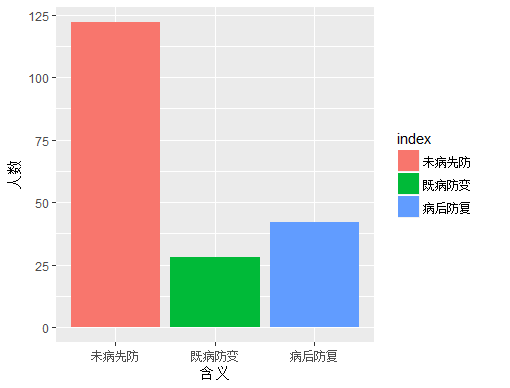
\includegraphics[scale=0.5]{./stats/hanyi.png}
\end{figure}
    \end{column}
    \begin{column}{0.6\textwidth}
        \begin{figure}[h]
            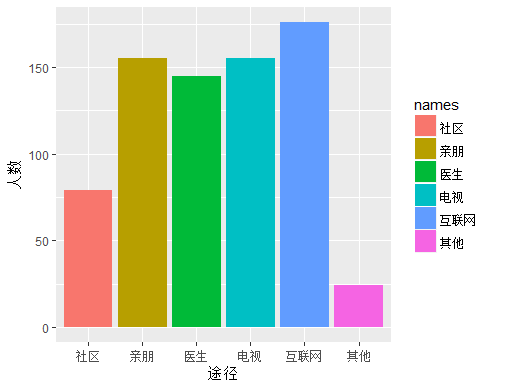
\includegraphics[scale=0.5]{./stats/ways.png}
        \end{figure} 
    \end{column}
\end{columns}

    \begin{columns}
    \begin{column}{0.5\textwidth}
        \begin{figure}[h]
            \caption{知识--态度--性别}
            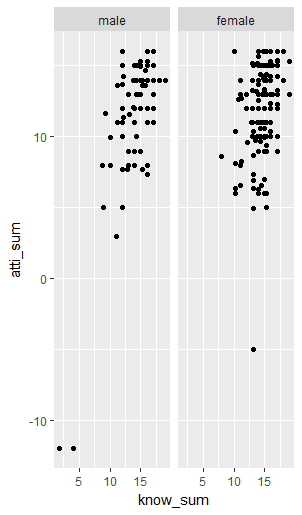
\includegraphics[scale=0.5]{./stats/know_sex.png}
            
        \end{figure}
           
    \end{column}
    \begin{column}{0.5\textwidth}
        \begin{figure}[h]
            \caption{知识--态度--收入}
           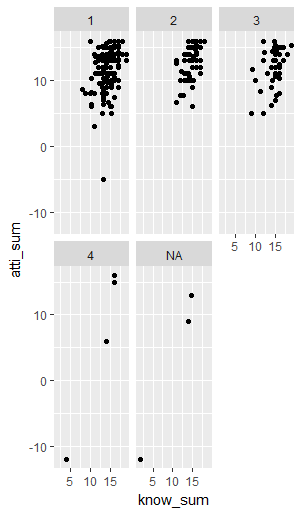
\includegraphics[scale=0.5]{./stats/know_income.png}
           
       \end{figure}
    \end{column}
\end{columns}

    \begin{columns}
    \begin{column}{0.5\textwidth}
        \begin{figure}[h]
             \caption{知识--态度--教育}
            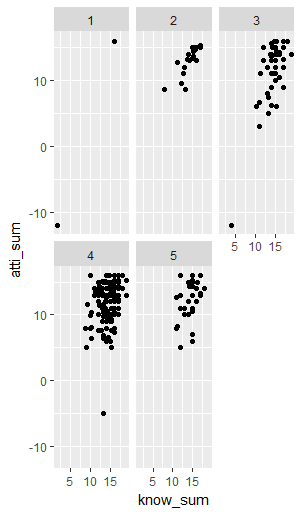
\includegraphics[scale=0.5]{./stats/know_grad.png}
           
        \end{figure}
        
    \end{column}
    \begin{column}{0.5\textwidth}
        \begin{figure}[h] 
            \caption{知识--态度--年龄}
            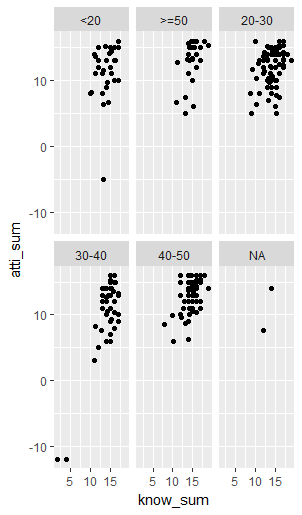
\includegraphics[scale=0.5]{./stats/know_age.png}
        \end{figure}
    \end{column}
\end{columns}

    \begin{columns}
    \begin{column}{0.5\textwidth}
        \begin{figure}[h]
            \caption{知识--行为--性别}
            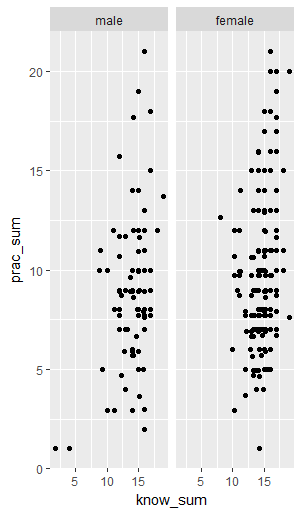
\includegraphics[scale=0.5]{./stats/prac_sex.png}
            
        \end{figure}
        
    \end{column}
    \begin{column}{0.5\textwidth}
        \begin{figure}[h]
            \caption{知识--行为--收入}
            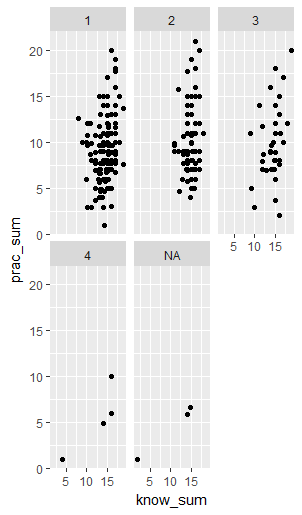
\includegraphics[scale=0.5]{./stats/prac_income.png}
            
        \end{figure}
    \end{column}
\end{columns}

    \begin{columns}
    \begin{column}{0.5\textwidth}
        \begin{figure}[h]
            \caption{知识--行为--教育}
            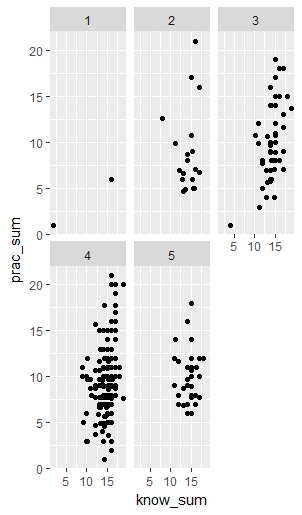
\includegraphics[scale=0.4]{./stats/prac_grad.png}
            
        \end{figure}
        
    \end{column}
    \begin{column}{0.5\textwidth}
        \begin{figure}[h] 
            \caption{知识--行为--年龄}
            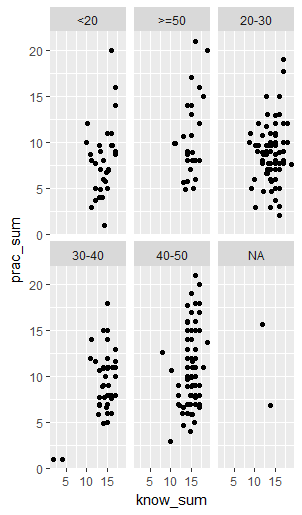
\includegraphics[scale=0.4]{./stats/prac_age.png}
        \end{figure}
    \end{column}
\end{columns}
    \begin{columns}
    \begin{column}{0.6\textwidth}
        \begin{figure}[h]
            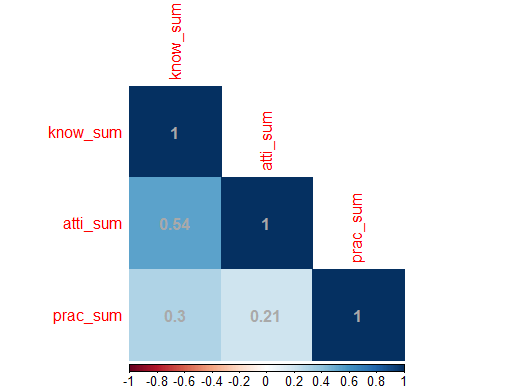
\includegraphics[scale=0.5]{./stats/corr.png}
            \caption{Pearson相关系数}
        \end{figure}
    \end{column}
    \begin{column}{0.6\textwidth}
        \begin{figure}[h]
            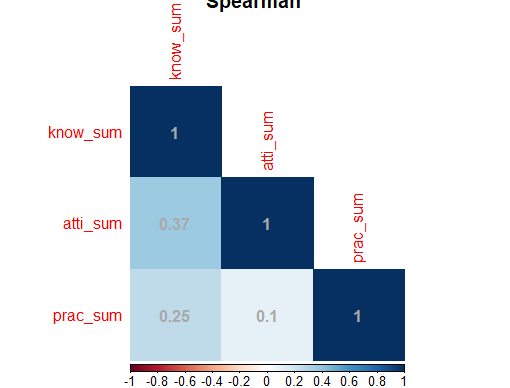
\includegraphics[scale=0.5]{./stats/cor_spearman.png}
            \caption{Spearman相关系数}
        \end{figure} 
    \end{column}
\end{columns}

\begin{exampleblock}{信而不行的原因}
    \begin{enumerate}
        \item 可能部分受调查者身体健康,没有就医或者保健的行动欲望
        \item 受调查者认为平常获取的养生信息可信度不高,半信半疑之间,不会付诸实际行动
        \item 受调查者意志力不高,无法执行养生做法
    \end{enumerate}
\end{exampleblock}
\end{frame}
\section{干预平台设计}
\setbeamercolor{background canvas}{bg=matblue}
\setbeamercolor{normal text}{fg=white}
\begin{frame}[plain, b]

\centering
\huge \textcolor{white}{如何实验?}
\normalsize

\vspace*{\fill}


\end{frame}
\setbeamercolor{background canvas}{bg=white}
\setbeamercolor{normal text}{fg=black}
\begin{frame}{实验设计模式}
\begin{figure}[h]
    \centering
    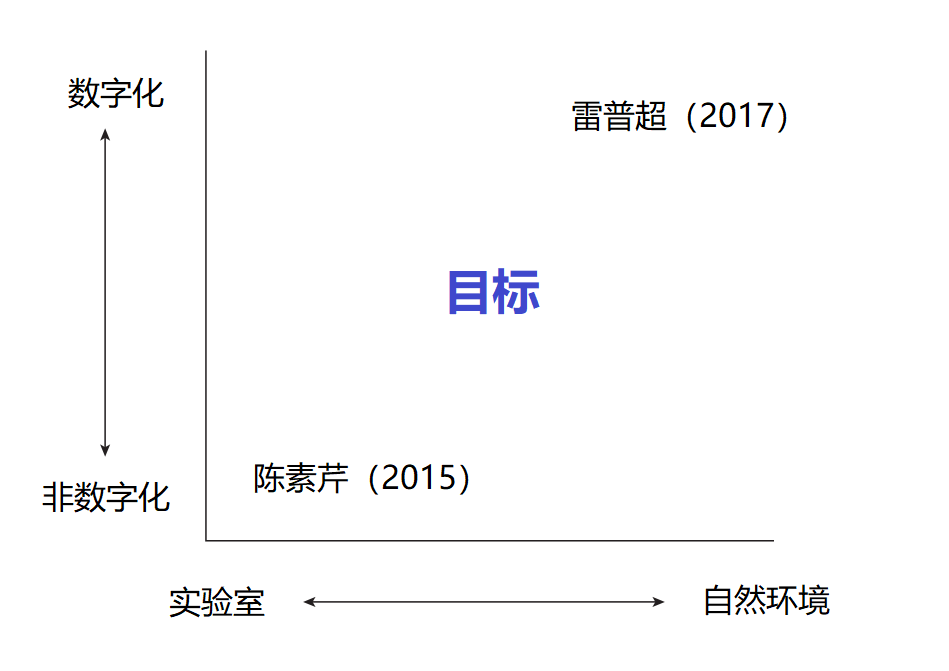
\includegraphics[scale=0.24]{digital.png}
    \caption{Source: Bit By Bit }
\end{figure}
\end{frame}
\begin{frame}{微信健康传播}
\begin{columns}
    \begin{column}{0.5\textwidth}
\begin{block}{微信公众平台优点}
\begin{itemize}
    \item 使用基数大;根据《2017年微信经济数据报告》,截至2017年底微信公众号已超过1000万个。
    \item 研究成本低,便于数据追踪和收集
    \item 数据更加真实,获取实验室环境难以得到的数据。
\end{itemize}
\end{block}
    \end{column}
\begin{column}{0.5\textwidth}
\begin{figure}[h]
    
\includegraphics[scale=0.3]{weixin.jpg}
\end{figure}
\end{column}
\end{columns}
\end{frame}

\begin{frame}{实验设计}
\begin{columns}
    \begin{column}{0.5\textwidth}
\begin{exampleblock}{研究变量}
    \begin{itemize}
        \item 分类变量:性别、年龄、收入、教育水平、职业、婚姻状况、慢病情况
        \item 连续变量:知识、信念、行为三维度得分、健康水平(SF-36量表得分)
        \item 终端变量:地理位置、阅读量、时间分析
    \end{itemize}
\end{exampleblock}
    \end{column}
\begin{column}{0.5\textwidth}
\begin{alertblock}{过程控制策略}
    \begin{enumerate}
        \item 统一招募标准 
        \item 随机化指定分组
        \item 使用tag管理分组
         \item 固定推送时间
        \item 每周投票/测试互动
        \item 前测和终测
    \end{enumerate}
\end{alertblock}
\end{column}
\end{columns}
\end{frame}

\begin{frame}{内容选择}
\begin{columns}
    \begin{column}{0.5\textwidth}
    \begin{block}{中医系列}
        \begin{itemize}
            \item 古人世界观、中医基本概念(30)
            \item 常见中药的介绍(20)
            \item 病案分析(15)
        \end{itemize}
    \end{block}
\end{column}
\begin{column}{0.5\textwidth}
    \begin{block}{养生系列}
        \begin{enumerate}
            \item 治未病饮食调理
            \item 治未病穴位保健
            \item 治未病运动功法
            \item 治未病精神调养
            \item 治未病热点专题
        \end{enumerate}
    \end{block}
\end{column}
\end{columns}
\end{frame}

\begin{frame}{平台预览}
    \begin{columns}
    \begin{column}{0.4\textwidth}
        \begin{figure}[h]
            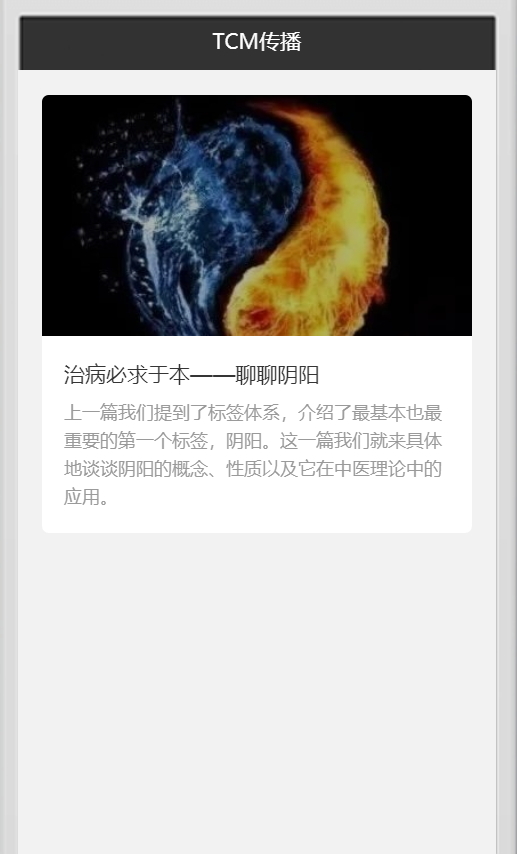
\includegraphics[scale=0.2]{wenzhang2.png}
            \caption{封面预览}
        \end{figure}
    \end{column}
    \begin{column}{0.4\textwidth}
        \begin{figure}[h]
            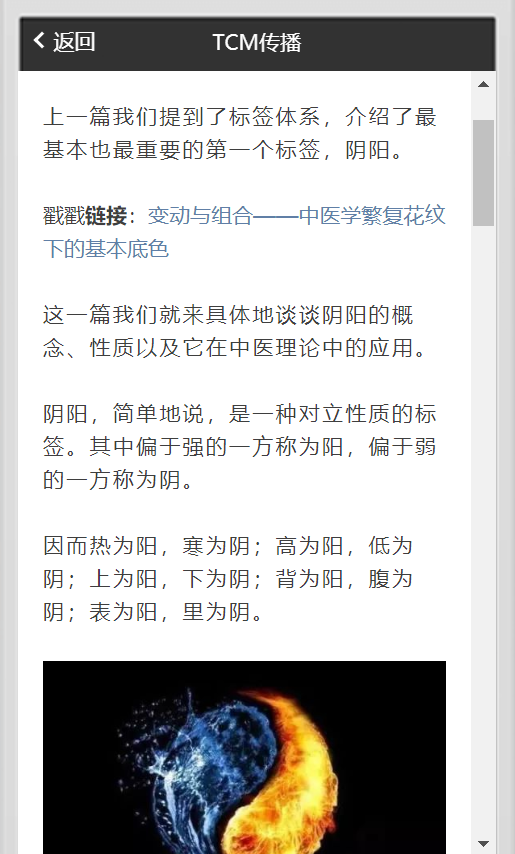
\includegraphics[scale=0.2]{wenzhang.png}
            \caption{图文预览}
        \end{figure} 
    \end{column}
\begin{column}{0.4\textwidth}
           \begin{figure}[h]
       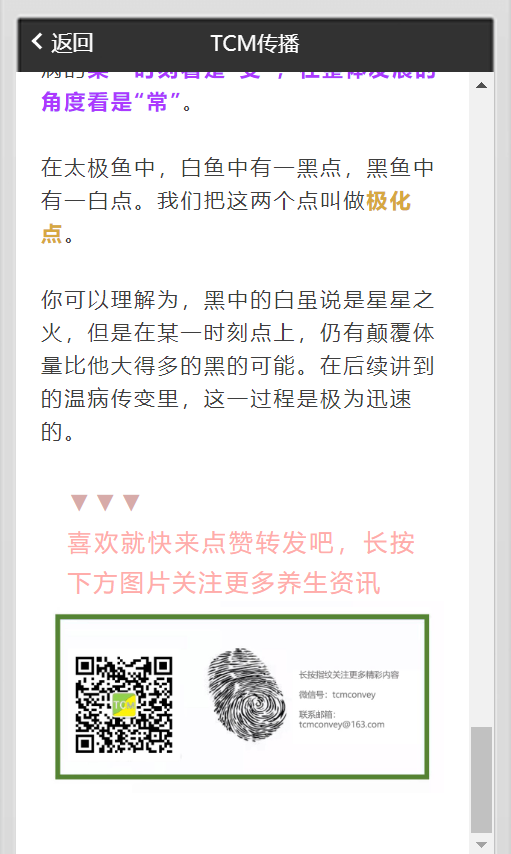
\includegraphics[scale=0.2]{wenzhang3.png}
       \caption{图文预览}
   \end{figure} 
\end{column}
\end{columns}
\end{frame}